%%%%%%%%%%%%%%%%%%%%%%%%%%%%%%%%%%%%%%%%%%%%%%%%%%%%%%%%%%%%%%%%%%%%%%%%%%%%%%%%
\chapter{Разработка метода интеллектуального обнаружения клонов}
%%%%%%%%%%%%%%%%%%%%%%%%%%%%%%%%%%%%%%%%%%%%%%%%%%%%%%%%%%%%%%%%%%%%%%%%%%%%%%%%
В данном разделе приводится подробное описание предлагаемого интеллектуального метода обнаружения клонов. А именно, приводится общая структура процесса обнаружения клонов, описываются основные этапы предложенного метода, раскрываются задачи, решаемые на данных этапах, приводятся необходимые алгоритмы. 
%%%%%%%%%%%%%%%%%%%%%%%%%%%%%%%%%%%%%%%%%%%%%%%%%%%%%%%%%%%%%%%%%%%%%%%%%%%%%%%%
\section{Общая схема алгоритма}
%%%%%%%%%%%%%%%%%%%%%%%%%%%%%%%%%%%%%%%%%%%%%%%%%%%%%%%%%%%%%%%%%%%%%%%%%%%%%%%%
Предлагаемый метод состоит из следующих основных этапов:
\begin{enumerate}
\setlength\itemsep{0mm}
\item предобработка
\item преобразование
\item обучение НС
\item обнаружение клонов
\item постобработка
\end{enumerate}

В рамках данного метода, на первом этапе, исходный код программы представляется в виде синтаксического дерева. Далее из него извлекаются поддеревья, связанные с функциями или методами классов, которые затем преобразуются в последовательности токенов. Перед последующим преобразованием осуществляется фильтрация и нормализация поддеревьев. Иными словами, удаляются не интересующие нас элементы.

На следующем этапе производится создание векторного представления токенов. С его помощью производится последующее обучение нейронной сети и анализ исходного кода на наличие программных клонов.

Далее следует процесс обучения нейронной сети. В том случае, когда сеть уже обучена, на этом этапе будет производиться поиск клонов с помощью этой сети.

На последнем этапе из всех обнаруженных клонов формируются клоновые классы, которые, в последствии и будут представлены пользователю. Общая структура процесса обнаружения клонов представлена на рисунке~\ref{fig:struct}.

\begin{figure}[htbp]
\centering
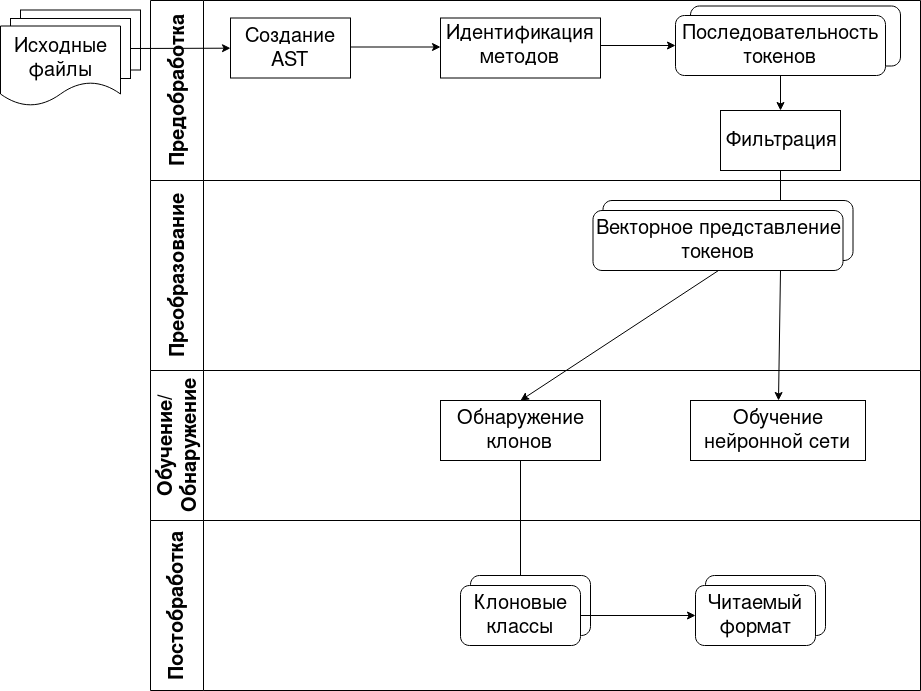
\includegraphics[width=3in]{struct.png}
\caption{Общая структура процесса обнаружения клонов}
\label{fig:struct}
\end{figure}

%%%%%%%%%%%%%%%%%%%%%%%%%%%%%%%%%%%%%%%%%%%%%%%%%%%%%%%%%%%%%%%%%%%%%%%%%%%%%%%%
\section{Предобработка}

На данном этапе, с помощью анализатора, основанного на части среды разработки (IDE Intellij IDEA community), производится представление исходного кода программы в виде AST. После чего, из полученного дерева выделяются только те поддеревья, которые относятся к методам или функциям. Такой поиск осуществляется посредством обхода в глубину всех вершин AST. В случае обнаружения вершины искомого типа, дальнейший спуск в данную ветку не осуществляется.

\nomenclature{IDE}{Integrated Development Environment}

Следующим этапом полученные поддеревья преобразуются в последовательности токенов путем того же обхода в глубину всех их вершин. После чего производится фильтрация этих последовательностей. Производимая фильтрация позволяет исключить влияние незначительных отличий фрагментов исходного кода друг от друга. В рамках данного подхода фильтрации подвергаются токены следующих типов:
\begin{itemize}
\setlength\itemsep{0mm}
\item комментарии различного типа
\item элементы форматирования
\item списки параметров
\end{itemize}

Обычно, для обнаружения клонов выше клонов I типа, необходимо производить анонимизацию токенов. Однако, в нашем методе, нейронная сеть будет сравнивать типы токенов. Из этого можно сделать вывод о ненадобности анонимизации. Таким образом, процесс фильтрации - последний процесс на этапе предобработки.
%%%%%%%%%%%%%%%%%%%%%%%%%%%%%%%%%%%%%%%%%%%%%%%%%%%%%%%%%%%%%%%%%%%%%%%%%%%%%%%%

\section{Преобразование}

На данном этапе производится преобразование полученных последовательностей токенов в их векторное представление. Данное преобразование производится с помощью модели Миколова - Word2Vec~\cite{word2vec}. Данная модель включает в себя набор алгоритмов расчета векторных представлений слов, предполагая семантическую близость слов используемых в похожих контекстах.

Рассматриваемая модель в своей работе использует нейронную сеть прямого распространения. В Word2Vec существуют два алгоритма обучения: CBOW (Continuous Bag of Words) и Skip-gram (рис. \ref{fig:word2vec}).

\nomenclature{CBOW}{Continuous Bag of Words}

CBOW и Skip-gram — это нейросетевые архитектуры, которые описывают, как именно нейросеть «учится» на данных и «запоминает» представления слов. Принципы у обоих архитектур разные. Принцип работы CBOW — предсказывание слова при данном контексте, а Skip-gram наоборот — предсказывается контекст при данном слове.

\begin{figure}[htbp]
\centering
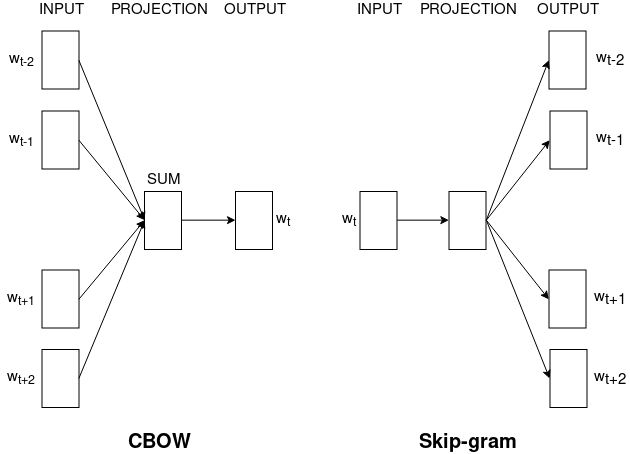
\includegraphics[width=3.5in]{word2vec.png}
\caption{Подходы к обучению Word2Vec}
\label{fig:word2vec}
\end{figure}

В данном подходе используется алгоритм Skip-gram. Как уже говорилось ранее, цель обучения Skip-gram модели - найти такие представления слов, которые будут полезны для предсказания контекста в предложении или документе. Формально, при заданной последовательности обучающих слов \(w_1, w_2, w_3,...,w_T\) целью обучаемой модели является максимизация средней логарифмической вероятности (\ref{eq:word2vec_log})

\begin{equation}
\label{eq:word2vec_log}
\frac{1}{T}\sum_{t=1}^{T}\sum_{-c \leq j \leq c,j\neq0}\log p(w_{t+j}|w_t)
\end{equation}

, где \(c\) - размер обучающего контекста (который может быть функцией центрального слова \(w_t\))~\cite{word2vec}.

Таким образом, после выполнения данного этапа, были получены векторные представления для каждого токена.
%%%%%%%%%%%%%%%%%%%%%%%%%%%%%%%%%%%%%%%%%%%%%%%%%%%%%%%%%%%%%%%%%%%%%%%%%%%%%%%%
\section{Обучение и использование нейронной сети}

\subsection{Выборка данных}

В рамка предлагаемого метода обнаружение программных клонов осуществляется при помощи нейронных сетей. Для корректного использования сетей их необходимо обучить. В данной секции будет рассматриваться этап обучения нейронной сети.

Одним из самых важных элементов в обучении нейронных сетей является набор обучающих данных. В открытом доступе, для данной задачи, подходящих наборов данных практически нет. Использование результатов других утилит, в качестве набора данных, не позволит объективно оценить предлагаемый подход, так как такое решение приведет к копированию функциональности таких инструментов. В связи с чем было принято решение разработки простого «мутатора» для генерации обучающего набора данных.

Основная задача разрабатываемого «мутатора» заключается в генерации различных программных клонов I-III типа. При этом, сгенерированные клоны не обязаны быть корректными с точки зрения компилятора.

Общая структура работы «мутатора» приведена на рисунке~\ref{fig:mut_stages}. Разработанный «мутатор» позволяет сгенерировать обучающую выборку данных. Однако, качество такой выборки не самое высокое и использовать ее можно как второстепенную.

\begin{figure}[htbp]
\centering
\includegraphics[width=\textwidth]{mut_stages.png}
\caption{Общая структура «мутатора»}
\label{fig:mut_stages}
\end{figure}

В качестве основной обучающей и тестовой выборки был выбран набор данных BigCloneBench~\cite{bcb}. Данная выборка представляет из себя коллекцию, состоящую из 8 млн проверенных программных клонов и 25 тыс. Java систем с открытым исходным кодом. BigCloneBench содержит как внутрипроектные, так и межпроектные программные клоны четырех типов~\cite{bcb}.

Главным преимуществом данной выборки является ее независимое создание от инструментов поиска клонов. Создание выборки таким образом позволяет избежать копирования функциональности существующих инструментов. 

Как было упомянуто ранее, в предлагаемом методе будут использоваться рекуррентные нейронные сети. Однако, они обладают недостатком, который заключается в потере информации со временем. Такой недостаток может быть легко устраним при использовании сетей с долгой краткосрочной памятью (LSTM). В LSTM-сетях внутренние нейроны «оборудованы» сложной системой так называемых ворот (gates), а также концепцией клеточного состояния (cell state), которая и представляет собой некий вид долгосрочной памяти. Ворота же определяют, какая информация попадет в клеточное состояние, какая сотрется из него, и какая повлияет на результат, который выдаст РНС на данном шаге~\cite{siam}.

\nomenclature{LSTM}{Long Short-Term Memory}
\nomenclature{РНС}{Рекуррентная Нейронная Сеть}

\begin{figure}[htbp]
\centering
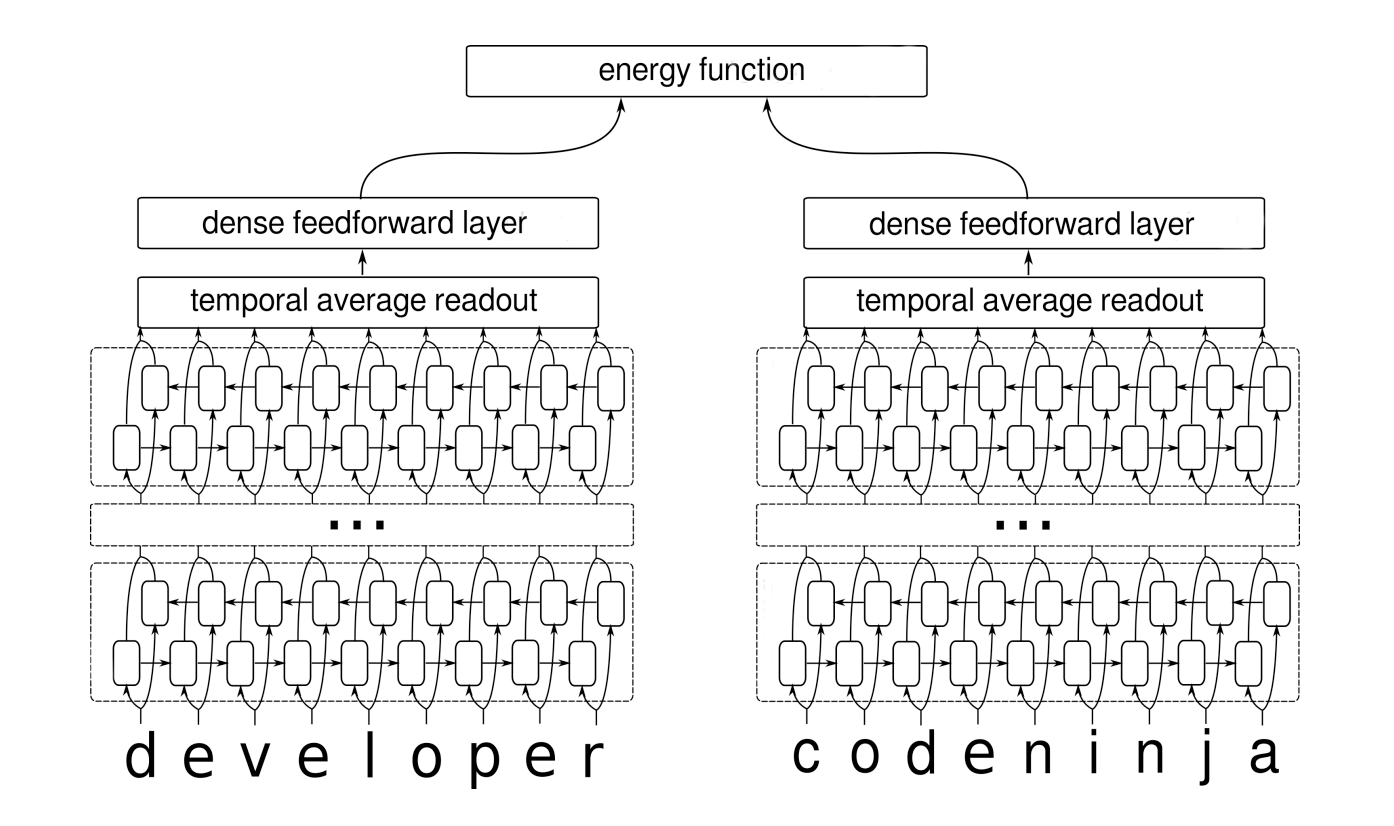
\includegraphics[width=\textwidth]{siam.png}
\caption{Сиамская нейронная сеть}
\label{fig:siam_mod}
\end{figure}

\subsection{Сиамская нейронная сеть}

В качестве архитектуры основной нейронной сети была выбрана, так называемая, Сиамская архитектура РНС. Такая архитектура применяется для оценки семантической схожести предложений. Используемая архитектура состоит из двух LSTM сетей со связанными весами, каждая из которых обрабатывает одно из предложений в заданной паре (рис.~\ref{fig:siam_mod}). Данная модель использует LSTM для чтения векторных представлений слов каждого входного предложения и использует свое окончательное скрытое состояние в качестве векторного представления предложений. Впоследствии, сходство между этими представлениями используется как предиктор семантического подобия~\cite{siam}.

Обучающая выборка для Сиамской сети состоит из триплетов \(x_1, x_2, y\), где \(x_1\) и \(x_2\) представляют из себя сравниваемые последовательности, а \(y \in \{0,1\}\) определяет сходство \(x_1\) и \(x_2\) (\(y = 1\)) или их различие (\(y = 0\)). Целью обучения является уменьшение дистанции между схожими парами и ее увеличение между различными.

Обучение сети производится с помощью использования контрастного коэффициента потерь и квадратичной регуляции \(l_2-norm\), что приводит к следующей целевой функции обучения:

\begin{equation}
\label{eq:contrastive}
L(w)=\frac{\lambda}{2}\|w\|_2^2+\frac{1}{2N}\sum_{(i,j) \in D}y_{ij}d_{ij}^2+(1-y_{ij}) max(1-d_{ij}^2,0)
\end{equation}

, где \(w\) - веса НС, \(D\) - набор обучающих пар, \(d_{ij}^2\) - квадратичное \(l_2\) расстояние между \(i\) и \(j\) последовательностями (рассчитанное между двумя последними слоями Сиамской НС), a \(y_{ij} \in {0,1}\) - как и было рассмотрено ранее - значение отвечающее за сходство/различие последовательностей~\cite{siam}.

\subsection{Sequence-to-Sequence}

В предлагаемом подходе программные клоны будут определяться на уровне методов. Так как методы могут быть разных размеров, то и их векторные представления могут быть также разных размеров. Существует два способа приведения представлений методов к единому размеру:

\begin{itemize}
\setlength\itemsep{0mm}
\item Выбор максимального размера и дополнения нулями до него
\item Использование модели sequence-to-sequence	(seq2seq)
\end{itemize}

В рассматриваемом методе была использована модель seq2seq. Данная модель пользуется большим успехом в различных задачах, например: распознавание речи, машинный перевод, обобщение текстов и т.п.

Суть такой модели заключается в использовании LSTM для считывания входной последовательности небольшими фрагментами до получения большого векторного представления с фиксированной размерностью. Затем используется другая LSTM для извлечения выходной последовательности из этого вектора (рис. \ref{fig:seq2seq})~\cite{seq2seq}. В качестве необходимого представления с фиксированным размером было использовано значение скрытой ячейки на последнем этапе развертывания кодировщика (thought vector на рис. \ref{fig:seq2seq}).

\begin{figure}[htbp]
\centering
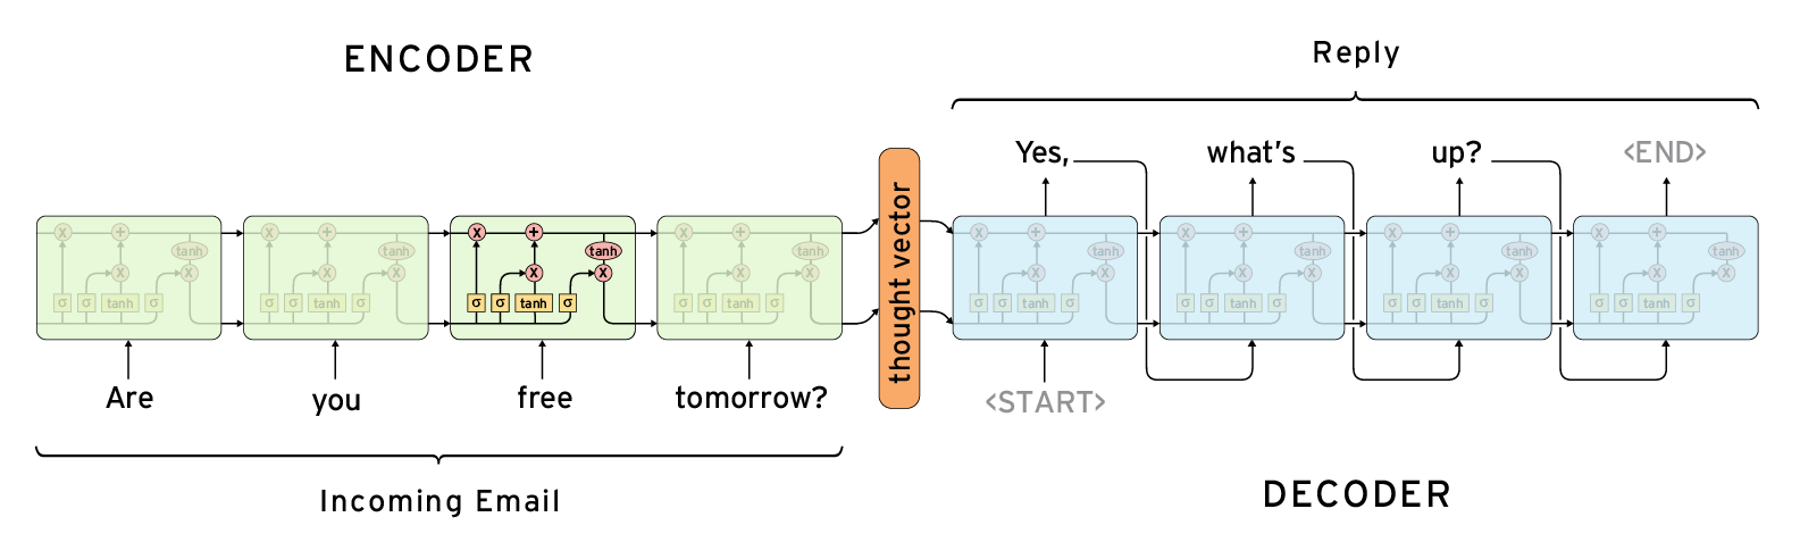
\includegraphics[width=\textwidth]{seq2seq.png}
\caption{Sequence-to-sequence}
\label{fig:seq2seq}
\end{figure}

Несмотря на тот факт, что в предлагаемом методе используется только часть модели seq2seq, необходимо проводить ее полное обучение. В качестве входных данных кодировщику и декодировщику подаются одинаковые вектора. Таким образом, seq2seq пытается привести входные данные кодировщика к фиксированному вектору, а затем - этот вектор к данным декодировщика. Иными словами, суть обучения заключается в увеличении логарифмической вероятности правильного перевода \(T\) с учетом исходного предложения \(S\):

\begin{equation}
\frac{1}{|D|}\sum_{(T,S) \in D} log_p(T|S)
\end{equation}

, где \(D\) - обучающий набор данных~\cite{seq2seq}.

\section{Постобработка}

Финальный этап предлагаемого метода - постобработка. Суть данного этапа заключается в приведении результатов в компактном и воспринимаемом человеком формате. Без данного этапа результат работы сети выглядит как набор векторных представлений с бинарным ответом о схожести двух методов. Таким образом, данный этап состоит из двух частей:

\begin{itemize}
\setlength\itemsep{0mm}
\item Создание клоновых классов (Компактность)
\item Вывод пути метода и его расположение в файле (номера строк начала метода и его конца) (Воспринимаемость)
\end{itemize}
